\subsection{Введение}
\subsubsection{Назначение}
Целью данного документа является создание социальной сети с числом активных
пользователей в более чем 100 млн.

\subsubsection{Конвенции в документа}
\begin{itemize}
\item HTML (HyperText Markup Language): Язык разметки, используемый для создания структуры веб-страницы.
\item CSS (Cascading Style Sheets): Язык стилей, который определяет внешний вид элементов HTML на веб-странице.
\item Chrome: Веб-браузер, разработанный компанией Google.
\item Safari: Веб-браузер, разработанный компанией Apple.
\item PHP: Язык программирования общего назначения, часто используемый для разработки веб-приложений и динамических сайтов.
\item JavaScript: Язык программирования, который обеспечивает интерактивность на веб-страницах.
\item MySQL: Система управления реляционными базами данных (СУБД), часто используемая в веб-разработке для хранения данных.
Apache Server: Веб-сервер, который обрабатывает запросы от клиентов и доставляет веб-страницы на их устройства.
\item ES5 (ECMAScript 5): Стандарт JavaScript, в котором определены основные возможности и функции языка.
\item SLA (Service Level Agreement): Документ, определяющий уровень обслуживания и обязательства между поставщиком услуг и клиентом.
\item Backup: Копии данных, созданные для обеспечения их сохранности и восстановления в случае потери или повреждения оригинальных данных.
\item HTTPS (HyperText Transfer Protocol Secure): Протокол передачи данных в сети Интернет, обеспечивающий защищенное соединение с использованием шифрования.
\item Беседа:
  Беседа представляет собой интерактивное средство общения между двумя или более пользователями. Она может включать текстовые сообщения, мультимедийные файлы.
\item Публикация:
   Публикация представляет собой контент, размещенный пользователем в его профиле или на общедоступной странице социальной сети. Это может быть текстовый пост, изображение, видео или другой мультимедийный контент, который доступен для просмотра другим пользователям.
 \item Сообщество:
 Сообщество представляет собой группу пользователей, объединенных общими интересами, целями или характеристиками. Сообщество включает в себя группу пользователей, подписанных на определенную тематику.
\item Новость:
   Новость представляет собой информационный материал, который размещается в социальной сети.
\item Стена:
   Стена представляет собой главную страницу пользователя в социальной сети, на которой отображается его активность, публикации, комментарии и другая информация. Она также может содержать контент, опубликованный друзьями или сообществами, за которыми следит пользователь.
 \item Интересы пользователя:
  Интересы пользователя представляют собой тематические области, темы или ключевые слова, которые отражают его предпочтения, хобби, профессиональные интересы и другие аспекты жизни.  Определяются по лайкам, поставленными пользователем.
\item Лайк (Like) - это функция или элемент в социальных сетях, который позволяет пользователям выразить свою положительную реакцию на контент или сообщение, опубликованное другим пользователями. Нажатие на кнопку <<Лайк>> позволяет пользователю показать свое одобрение или заинтересованность в определенном контенте.
\item Сжатие данных:
  Сжатие данных представляет собой процесс уменьшения размера цифровых данных для экономии места на серверах и ускорения передачи данных по сети. Сжатие данных может применяться к мультимедийному контенту, такому как изображения и видео, для более эффективного хранения и передачи данных.
\item Незаконный контент:
  Незаконный контент представляет собой информацию, контент или материалы, нарушающие законодательство или правила социальной сети. Это может включать в себя контент, нарушающий авторские права, содержащий ненормативную лексику, пропагандирующий насилие или содержащий запрещенные материалы.

\item Корректное отображение интерфейса:
  Корректное отображение интерфейса означает, что пользовательский интерфейс социальной сети должен быть отображен на экране пользователя без ошибок, искажений.
\end{itemize}
\subsubsection{Предполагаемая аудитория и предложения по чтению}
Данный документ относится к социальной сети <<ВКонтакте>>.
Он предназначается для чтения программистами, менеджерами, тестировщиками, аналитиками, маркетологами.

\subsubsection{Классы и характеристики пользователей}
\begin{enumerate}
  \item Пользователь. Пользователь -- конечный потребитель социальной
    сети, желающий использовать ее для связи с родными, друзьями и знакомыми, просматривать ленту новостей, просматривать и отправлять фото-, видео- и аудио-контент.
  \item Владелец сайта. Владелец сайта желает использовать социальную сеть
  для получения прибыли. Кроме того, владелец сайта заинтересован в соблюдении
    социальной сетью всех законов Российской Федерации.
  \item Модерация сайта.
    Модерация сайта просмтаривает публикации пользователей и сообществ на предмет
    соответствия закону Российской Федерации.
  \item Техническая поддержка.
    Техническая поддержка отвечает пользователю на сообщения об ошибках и
    помогает пользователю в случае трудностей.
\end{enumerate}

\subsubsection{Масштаб проекта}
Социальная сеть ВКонтакте предоставляет пользователям возможность связываться на расстоянии посредством текстовых-, аудио-, фото-, и видео-коммуницирования.
Кроме того, платформа может рассматриваться как хостинг-площадка для аудио- и видео-материалов.

\subsubsection{Ссылки}

\subsection{Описание продукта}
\subsubsection{Функциональность продукта}
\begin{itemize}
  \item Регистрация в сети
  \item Отправка текстовых сообщений
  \item Отправка видео сообщений
  \item Отправка голосовых сообщений
  \item Отправка фото сообщений.
  \item Создание групп, сообществ, бесед
  \item Ведение блога на своей странице
\end{itemize}

\subsubsection{Условия эксплуатации}
Социальная сеть ВКонтакте требует
для своей работы Apache Server и базу данных MySQL.

\subsubsection{Ограничения на проектирование и реализацию}
Проект должен быть реализован с помощью языков программирования PHP, HTML, CSS и JavaScript.
Проект должен использовать базу данных MySQL.
Серверная часть сайта должна обеспечивать
корректную работу при 25'000 запросов в секунду.

\subsubsection{Документация пользователя}
Для работы с данным сайтом нет нужды в дополнительной литературе.

\subsection{Требования}
\subsubsection{Функциональные требования}
\paragraph{Требования пользователя}
\begin{enumerate}
  \item FRU1. Система должна предоставлять возможность зарегистрироваться в сети
  \item FRU2. Система должна предоставлять возможность блокировать нежелательных пользователей
  \item FRU3. Система должна предоставлять возможность отправлять другим пользователям сообщения.
  \item FRU4. Система должна предоставлять пользователям вомзожность создавать на своей странице публикации, содержащие текстовый, фото-, аудио- и видео-контент.
  \item FRU5. Система должна предоставлять возможность создавать беседы и сообщества.
  \item FRU6. Система должна предоставлять пользователям возможность создавать публикации от имени сообщества.
  \item FRU7. Система должна предоставлять возможность отмечать понравившиеся публикации, комментарии и фотографии на страницах других пользователей и на страницах сообществ.
  \item FRU8. Система должна предоставлять возможность указывать информации о себе на своей странице.
  \item FRU9. Система должна предоставлять возможность просматривать ленту публикаций.
  \item FRU10. Система должна предоставлять возможность оставить обратную связь, в том числе для получения помощи со стороны технической поддержки.
\end{enumerate}

\paragraph{Требования владельца сайта}
\begin{enumerate}
\item FRO1. Система должна предоставлять возможность блокировать пользователя.
\item FRO2. Система должна требовать от пользователя указание номера телефона.
\item FRO3. Система должна оптимизировать картинки, видео и аудио с помощью сжатия.
\item FRO4. Система должна блокировать незаконный контент.
\item FRO5. Система должна предоставлять возможность выгрузить переписку определенного пользователя
  путем нажатия на красную кнопку <<\texttt{РАСКРЫТЬ ТАЙНУ ПЕРЕПИСКИ}>>.
\end{enumerate}

\paragraph{Требования технической поддержки}
\begin{enumerate}
  \item FRS1. Система должна предоставлять возможность отвечать на вопросы пользователя, заданные с помощью
    формы обртаной связи.
\end{enumerate}

\paragraph{Требования модераторов}
\begin{enumerate}
  \item FRM1. Система должна предоставлять возможность блокировать пользователя.
\end{enumerate}


\subsubsection{Нефункциональные требования}
Интерфейсы пользователя:
\begin{enumerate}
\item Система должна поддерживать отображение сайта без нарушения работы функциональности и  дизайна в браузерах: Chrome 79+, Safari 11+, Mozilla 70+, Yandex Browser 21+ и иных браузерах с поддержкой HTML5, CSS2+ и ES5+.
\item Система должна поддерживать корректное отображение мобильной версии сайта 
\end{enumerate}

Требования к безопасности системы:

\begin{enumerate}
\item Система должна обновлять бэкапы базы данных каждые 2 недели.
\item Система должна обеспечивать время обработки запроса, которое не должно превышать 3 секунды при наличии у клиента интернета со скоростью не менее 10 Мбит/с.
\item Система должна предоставлять  безопасную передачу данных пользователей (использование протокола HTTPS)
\end{enumerate}

\subsubsection{Атрибуты требований}
\begin{longtable}{|l|p{3cm}|l|p{3cm}|p{4cm}|}
\hline
  \textnumero & Требование & Трудоемкость (в человекочасах) & Приоритет \\
\hline
1 & FRU1 & 40 & Must Have \\
\hline
2 & FRU2 & 20 & Could Have \\
\hline
3 & FRU3 & 20 & Must Have \\
\hline
4 & FRU4 & 40 & Should Have \\
\hline
5 & FRU5 & 80 & Should Have \\
\hline
6 & FRU6 & 40 & Should Have \\
\hline
7 & FRU7 & 80 & Could Have \\
\hline
8 & FRU8 & 40 & Could Have \\
\hline
9 & FRU9 & 30 & Should Have \\
\hline
10 & FRU10 & 60 & Could Have \\
\hline
\hline
11 & FRO1 & 40 & Must Have \\
\hline
12 & FRO2 & 10 & Must Have \\
\hline
13 & FRO3 & 80 & Should Have \\
\hline
14 & FRO4 & 160 & Must Have \\
\hline
\hline
15 & FRS1 & 80 & Should Have \\
\hline
16 & FRM1 & 40 & Should Have \\
\hline
\end{longtable}

\subsection{Риски}
\subsubsection{Функциональность продукта}
\begin{itemize}
\item Ресурсные риски:
    \begin{itemize}
        \item Нехватка людей на разработку/поддержку проекта.
          Этот считается активированным, если из изначальной команды разработчиков
          в 20 человек уйдет более 50\%.
          В случае этого риска предполагается увеличить заработные платы всем
          работникам для улучшения их удержания, открыть больше вакансий с более высокой зарплатой.
        \item Отсутствие финансирования
          Этот риск считается активированным если будет потрачено более 100 млн. рублей ($1/2$ бюджета)
          из общего бюджета компании.
          В случае этого риска предполагается взять кредит (если осталось более 10 млн. рублей)
          или объявить банкротство.
    \end{itemize}
\item Бизнес-риски:
    \begin{itemize}
        \item Отток клиентов к конкурентам.
          Этот риск считается активированным, когда количество активных пользователей за месяц (MAU)
          становится падает больше, чем на 25\% от предыдущего месяца.
          В случае этого риска предлагается увеличить бюджеты на рекламную кампанию.
    \end{itemize}
\item Технические риски:
        \begin{itemize}
        \item Ненадежность используемых сервисов, баз данных.
          Этот риск активируется в случае сбоев или поломок оборудования или программных средств.
          В случае этого риска предлагается быстро заменить неисправленное оборудование или
            использовать дублирующие сервисы.
    \end{itemize}
\item Юридические риски:
        \begin{itemize}
        \item Изменения в законодательстве, связанные с распространением информации.
          Этот риск считается активированным, если произошли изменения в законодательстве.
          В случае возникновения этого риска предлагается отправить изменения юридическому отделу на изучение.
        \item Невозможность использования веб-сайта в другие страны и регионы из-за политических конфликтов/санкций
          Этот риск считается активированным в случае политических кризисов, вооруженных конфликтов.
          В случае возникновения этого риска предлагается проконсультироваться с юридическим отделом.
    \end{itemize}
\item Форс-мажор. Этот риск считается активированным, если государство объявило форс-мажор.
  В случае форс мажора предлагается обратиться в страховую компанию.
\end{itemize}

\subsection{Прецеденты}
\begin{center}
  \begin{tabular}{|l|p{9cm}|}
  \hline
  \textbf{Прецедент} & Пользователь регистрируется в сети \\
  \hline
  \textbf{ID} & 1 \\
  \hline
  \textbf{Краткое описание} & Пользователь может зарегистрироваться в социальной сети \\
  \hline
  \textbf{Главный актер} & Пользователь\\
  \hline
  \textbf{Второстепенные актеры} & нет \\
  \hline
  \textbf{Предусловия} & у пользователя есть номер телефона \\
  \hline
  \textbf{Основной поток} & \begin{enumerate}
    \item Пользователь переходит на страницу регистрации
    \item Пользователь вводит свои данные: ФИО, номер телефона и пароль.
    \item Пользователь подтверждает свои данные с помощью sms.
  \end{enumerate} \\
  \hline
\end{tabular}
\end{center}

\begin{center}
  \begin{tabular}{|l|p{9cm}|}
  \hline
  \textbf{Прецедент} & Пользователь входит в сеть \\
  \hline
  \textbf{ID} & 2 \\
  \hline
  \textbf{Краткое описание} & Пользователь может войти в социальнюу сеть \\
  \hline
  \textbf{Главный актер} & Пользователь\\
  \hline
  \textbf{Второстепенные актеры} & нет \\
  \hline
  \textbf{Предусловия} & пользователь прошел регистрацию \\
  \hline
  \textbf{Основной поток} & \begin{enumerate}
    \item Пользователь переходит на страницу входа
    \item Пользователь вводит свои данные: номер телефона и пароль.
    \item Пользователь нажимает на кнопку <<Войти>>
  \end{enumerate} \\
  \hline
\end{tabular}
\end{center}

\begin{center}
  \begin{tabular}{|l|p{9cm}|}
  \hline
  \textbf{Прецедент} & Пользователь скроллит ленту новостей \\
  \hline
  \textbf{ID} & 3 \\
  \hline
  \textbf{Краткое описание} & Пользователь может просматривать ленту новостей, сформированной на основе подписок, рекомендаций и публикацией друзей \\
  \hline
  \textbf{Главный актер} & Пользователь\\
  \hline
  \textbf{Второстепенные актеры} & нет \\
  \hline
  \textbf{Предусловия} & Пользователь вошел в систему \\
  \hline
  \textbf{Основной поток} & \begin{enumerate}
    \item Пользователь переходит на основную страницу сайта
    \item Пользователь скроллит ленту и взаимодействует с постами (лайкает, пересылает)
  \end{enumerate} \\
  \hline
\end{tabular}
\end{center}

\begin{center}
  \begin{tabular}{|l|p{9cm}|}
  \hline
  \textbf{Прецедент} & Пользователь оформляет свою страницу \\
  \hline
  \textbf{ID} & 4 \\
  \hline
  \textbf{Краткое описание} & Пользователь может оформлять свою страницу, добавлять фотографии, создавать посты, указывать свои данные. \\
  \hline
  \textbf{Главный актер} & Пользователь\\
  \hline
  \textbf{Второстепенные актеры} & нет \\
  \hline
  \textbf{Предусловия} & Пользователь вошел в систему \\
  \hline
  \textbf{Основной поток} & \begin{enumerate}
    \item Пользователь переходит на страницу "о себе"
    \item Пользователь может создавать публикации (размещение фото-, видео-, файлов и текстов)
    \item Пользователь может перейти на страницу "настройки профиля"
    \item  Пользователь может добавлять, удалять информацию о себе (город проживания, место рождения, дата рождения, возраст, школа, вуз, интересы)
  \end{enumerate} \\
  \hline
\end{tabular}
\end{center}

\begin{center}
  \begin{tabular}{|l|p{9cm}|}
  \hline
  \textbf{Прецедент} & Пользователь отправляет сообщение\\
  \hline
  \textbf{ID} & 5 \\
  \hline
  \textbf{Краткое описание} & Пользователь имеет возможность отправлять сообщения другим пользователя(в том числе и группам). \\
  \hline
  \textbf{Главный актер} & Пользователь\\
  \hline
  \textbf{Второстепенные актеры} & другие пользователи или группы \\
  \hline
  \textbf{Предусловия} & Пользователь вошел в систему \\
  \hline
  \textbf{Основной поток} & \begin{enumerate}
    \item Пользователь переходит на страницу сообщений.
    \item Пользователь выбирает получателя.
    \item Пользователь выбирает тип отправляемого сообщения (аудио-, видео-, файл или обычный текст)
    \item Пользователь вводит необходимый текст.
    \item Пользователь нажимает кнопку отправки. 
    \item Другие пользователи или группы получают сообщение.
  \end{enumerate} \\
  \hline
\end{tabular}
\end{center}

\begin{center}
  \begin{tabular}{|l|p{9cm}|}
  \hline
  \textbf{Прецедент} & Пользователь блокирует нежелательных пользователей\\
  \hline
  \textbf{ID} & 6 \\
  \hline
  \textbf{Краткое описание} & Пользователь имеет возможность навсегда заблокировать нежелательного ему пользователя. \\
  \hline
  \textbf{Главный актер} & Пользователь\\
  \hline
  \textbf{Второстепенные актеры} & другие пользователи или группы \\
  \hline
  \textbf{Предусловия} & Пользователь успешно вошел в систему \\
  \hline
  \textbf{Основной поток} & \begin{enumerate}
    \item Пользователь переходит на страницу другого пользователя
    \item Пользователь выбирает "действия с пользователем"
    \item Пользователь выбирает "Добавить пользователя в черный список" 
  \end{enumerate} \\
  \hline
\end{tabular}
\end{center}

\begin{center}
  \begin{tabular}{|l|p{9cm}|}
  \hline
  \textbf{Прецедент} & Пользователь создает беседу \\
  \hline
  \textbf{ID} & 7 \\
  \hline
  \textbf{Краткое описание} & Пользователи имеют возможность создавать и присоединяться к беседам.\\
  \hline
  \textbf{Главный актер} & Пользователь\\
  \hline
  \textbf{Второстепенные актеры} & Другие пользователи или группы \\
  \hline
  \textbf{Предусловия} & Пользователь успешно вошел в систему \\
  \hline
  \textbf{Основной поток} & \begin{enumerate}
    \item Пользователь переходит на страницу сообщений.
    \item Пользователь выбирает "создать чат".
    \item Пользователь выбирает других пользователей, кто будет добавлен в данную беседу.
    \item Пользователь выбирает название беседы, фотографию  и описание.
    \item У пользователей появляется новая беседа на странице "чаты".
  \end{enumerate} \\
  \hline
\end{tabular}
\end{center}

\begin{center}
  \begin{tabular}{|l|p{9cm}|}
  \hline
  \textbf{Прецедент} & Владелец раскрывает тайну переписки \\
  \hline
  \textbf{ID} & 8 \\
  \hline
  \textbf{Краткое описание} & Владелец имеет возможность раскрыть тайну переписки пользователей.\\
  \hline
  \textbf{Главный актер} & Владелец\\
  \hline
  \textbf{Второстепенные актеры} & -- \\
  \hline
  \textbf{Предусловия} & Владелец находится в офисе \\
  \hline
  \textbf{Основной поток} & \begin{enumerate}
    \item Владелец спускается в подвал
    \item Владелец вставляет flash-накопитель в USB-разъем.
    \item Владелец нажимает на красную кнопку \texttt{РАСКРЫТЬ ТАЙНУ ПЕРЕПИСКИ}.
    \item Владелец извлекает flash-накопитель из USB-разъема.
  \end{enumerate} \\
  \hline
\end{tabular}
\end{center}

\begin{center}
  \begin{tabular}{|l|p{9cm}|}
  \hline
  \textbf{Прецедент} & Техподдержка отвечает на вопрос пользователя \\
  \hline
  \textbf{ID} & 9 \\
  \hline
  \textbf{Краткое описание} & Техподдержка имеет возможность ответить на вопросы пользователей, отправленные с помощью формы обратной связи. \\
  \hline
  \textbf{Главный актер} & Тех. поддержка \\
  \hline
  \textbf{Второстепенные актеры} & Пользователь \\
  \hline
  \textbf{Предусловия} & Пользователь отправил вопрос с помощью формы обратной связи \\
  \hline
  \textbf{Основной поток} & \begin{enumerate}
    \item Работник тех. поддержки переходит на страницу технической поддержки.
    \item Работник тех. поддержки выбирает вопрос пользователя
    \item Работник тех. поддержки отвечает на вопрос пользователя в текстовом элементе ввода.
    \item Работник тех. поддержки отправляет ответ.
  \end{enumerate} \\
  \hline
\end{tabular}
\end{center}

\begin{center}
  \begin{tabular}{|l|p{9cm}|}
  \hline
  \textbf{Прецедент} & Модерация удаляет незаконный контент \\
  \hline
  \textbf{ID} & 10 \\
  \hline
  \textbf{Краткое описание} & Модератор имеет возможность удалить обнаруженный незаконный контент. \\
  \hline
  \textbf{Главный актер} & Модератор \\
  \hline
  \textbf{Второстепенные актеры} & --  \\
  \hline
  \textbf{Предусловия} & Модератор обнаруживает незаконный контент \\
  \hline
  \textbf{Основной поток} & \begin{enumerate}
    \item Модератор анализирует незаконность контента.
    \item Модератор принимает решение об удалении контента.
    \item Модератор удаляет контент или помечает его как законный.
  \end{enumerate} \\
  \hline
\end{tabular}
\end{center}




\subsection{Диаграмма прецедентов}
\begin{figure}[H]
  \resizebox{\textwidth}{!}{% generated by Plantuml 1.2023.13      
\definecolor{plantucolor0000}{RGB}{0,0,0}
\definecolor{plantucolor0001}{RGB}{241,241,241}
\definecolor{plantucolor0002}{RGB}{24,24,24}
\begin{tikzpicture}[yscale=-1
,pstyle0/.style={color=black,line width=1.5pt}
,pstyle1/.style={color=plantucolor0002,fill=plantucolor0001,line width=0.5pt}
,pstyle2/.style={color=plantucolor0002,line width=0.5pt}
,pstyle3/.style={color=plantucolor0002,line width=1.0pt,dash pattern=on 7.0pt off 7.0pt}
,pstyle4/.style={color=plantucolor0002,fill=plantucolor0002,line width=1.0pt}
,pstyle5/.style={color=plantucolor0002,line width=1.0pt}
]
\draw[pstyle0] (496.01pt,6.602pt) -- (559.6065pt,6.602pt) arc(270:360:3.75pt)  -- (569.1065pt,31.6699pt) -- (910.21pt,31.6699pt) arc(270:360:2.5pt)  -- (912.71pt,1041.102pt) arc(0:90:2.5pt)  -- (496.01pt,1043.602pt) arc(90:180:2.5pt)  -- (493.51pt,9.102pt) arc(180:270:2.5pt) ;
\draw[pstyle0] (493.51pt,31.6699pt) -- (569.1065pt,31.6699pt);
\node at (497.51pt,8.602pt)[below right,color=black]{\textbf{vk.com}};
\draw[pstyle1] (703.1091pt,159.6058pt) ellipse (93.5191pt and 21.1038pt);
\node at (630.5915pt,149.3728pt)[below right,color=black]{Создание беседы};
\draw[pstyle1] (703.1087pt,256.6017pt) ellipse (193.5987pt and 41.1197pt);
\node at (524.5675pt,245.0678pt)[below right,color=black]{Блокировка нежелательных пользователей};
\draw[pstyle1] (703.1084pt,547.6037pt) ellipse (111.9584pt and 24.7917pt);
\node at (608.5725pt,537.3707pt)[below right,color=black]{Отправка сообщенеий};
\draw[pstyle1] (703.1065pt,637.5993pt) ellipse (138.1865pt and 30.0373pt);
\node at (582.6036pt,626.0653pt)[below right,color=black]{Оформление своей страницы};
\draw[pstyle1] (703.1117pt,723.5983pt) ellipse (92.9317pt and 20.9863pt);
\node at (631.3286pt,713.3654pt)[below right,color=black]{Просмотр ленты};
\draw[pstyle1] (703.1132pt,64.5986pt) ellipse (87.5832pt and 19.9166pt);
\node at (638.1562pt,54.3657pt)[below right,color=black]{Вход в систему};
\draw[pstyle1] (703.1106pt,462.6021pt) ellipse (113.2506pt and 25.0501pt);
\node at (607.0882pt,452.3691pt)[below right,color=black]{Регистрация в системе};
\draw[pstyle1] (703.1065pt,901.6013pt) ellipse (123.6465pt and 27.1293pt);
\node at (596.743pt,890.8149pt)[below right,color=black]{Пожаловаться на контент};
\draw[pstyle1] (703.1074pt,367.5975pt) ellipse (164.8274pt and 35.3655pt);
\node at (554.4604pt,356.0635pt)[below right,color=black]{Получение переписки пользователя};
\draw[pstyle1] (703.1085pt,809.6037pt) ellipse (136.2585pt and 29.6517pt);
\node at (584.6681pt,798.0697pt)[below right,color=black]{Обращение к тех. поддержке};
\draw[pstyle1] (703.114pt,995.6008pt) ellipse (149.644pt and 32.3288pt);
\node at (570.4343pt,984.0668pt)[below right,color=black]{Удаление незаконного контента};
\draw[pstyle1] (105.2543pt,516.572pt) ellipse (8pt and 8pt);
\draw[pstyle2] (105.2543pt,524.572pt) -- (105.2543pt,551.572pt)(92.2543pt,532.572pt) -- (118.2543pt,532.572pt)(105.2543pt,551.572pt) -- (92.2543pt,566.572pt)(105.2543pt,551.572pt) -- (118.2543pt,566.572pt);
\node at (48.74pt,568.072pt)[below right,color=black]{Пользователь};
\draw[pstyle1] (1023.2373pt,336.572pt) ellipse (8pt and 8pt);
\draw[pstyle2] (1023.2373pt,344.572pt) -- (1023.2373pt,371.572pt)(1010.2373pt,352.572pt) -- (1036.2373pt,352.572pt)(1023.2373pt,371.572pt) -- (1010.2373pt,386.572pt)(1023.2373pt,371.572pt) -- (1036.2373pt,386.572pt);
\node at (959.71pt,388.072pt)[below right,color=black]{Владелец сайта};
\draw[pstyle1] (105.2533pt,910.572pt) ellipse (8pt and 8pt);
\draw[pstyle2] (105.2533pt,918.572pt) -- (105.2533pt,945.572pt)(92.2533pt,926.572pt) -- (118.2533pt,926.572pt)(105.2533pt,945.572pt) -- (92.2533pt,960.572pt)(105.2533pt,945.572pt) -- (118.2533pt,960.572pt);
\node at (60.12pt,962.072pt)[below right,color=black]{Модератор};
\draw[pstyle1] (105.255pt,778.572pt) ellipse (8pt and 8pt);
\draw[pstyle2] (105.255pt,786.572pt) -- (105.255pt,813.572pt)(92.255pt,794.572pt) -- (118.255pt,794.572pt)(105.255pt,813.572pt) -- (92.255pt,828.572pt)(105.255pt,813.572pt) -- (118.255pt,828.572pt);
\node at (6pt,830.072pt)[below right,color=black]{Техническая поддержка};
\draw[pstyle3] (703.11pt,138.042pt) ..controls (703.11pt,122.062pt) and (703.11pt,106.422pt) .. (703.11pt,90.772pt);
\draw[pstyle4] (703.11pt,84.772pt) -- (699.11pt,93.772pt) -- (703.11pt,89.772pt) -- (707.11pt,93.772pt) -- (703.11pt,84.772pt) -- cycle;
\node at (664.61pt,103.012pt)[below right,color=black]{include};
\draw[pstyle3] (526.24pt,273.712pt) ..controls (473.93pt,269.012pt) and (421.46pt,252.782pt) .. (386.86pt,213.102pt) ..controls (313.71pt,129.212pt) and (501.9756pt,90.0967pt) .. (617.8356pt,74.2167pt);
\draw[pstyle4] (623.78pt,73.402pt) -- (614.3202pt,70.6612pt) -- (618.8263pt,74.0809pt) -- (615.4065pt,78.5871pt) -- (623.78pt,73.402pt) -- cycle;
\node at (330.01pt,195.102pt)[below right,color=black]{include};
\draw[pstyle3] (593.33pt,542.132pt) ..controls (556.9pt,536.362pt) and (517.51pt,525.542pt) .. (485.51pt,505.602pt) ..controls (423.8pt,467.162pt) and (409.98pt,444.032pt) .. (386.86pt,375.102pt) ..controls (370.8pt,327.222pt) and (337.07pt,248.962pt) .. (485.51pt,120.602pt) ..controls (521.73pt,89.282pt) and (567.3003pt,75.9705pt) .. (611.1203pt,69.7105pt);
\draw[pstyle4] (617.06pt,68.862pt) -- (607.5848pt,66.175pt) -- (612.1103pt,69.5691pt) -- (608.7161pt,74.0946pt) -- (617.06pt,68.862pt) -- cycle;
\node at (330.01pt,357.102pt)[below right,color=black]{include};
\draw[pstyle3] (574.08pt,626.612pt) ..controls (543.04pt,619.432pt) and (511.41pt,607.922pt) .. (485.51pt,589.602pt) ..controls (417.77pt,541.692pt) and (409.66pt,510.882pt) .. (386.86pt,431.102pt) ..controls (370.45pt,373.682pt) and (286.83pt,305.012pt) .. (485.51pt,120.602pt) ..controls (520.68pt,87.962pt) and (566.3338pt,74.5637pt) .. (610.4638pt,68.6137pt);
\draw[pstyle4] (616.41pt,67.812pt) -- (606.9562pt,65.0504pt) -- (611.4548pt,68.4801pt) -- (608.0252pt,72.9787pt) -- (616.41pt,67.812pt) -- cycle;
\node at (330.01pt,413.102pt)[below right,color=black]{include};
\draw[pstyle3] (610.7pt,726.632pt) ..controls (568.64pt,723.532pt) and (520.55pt,713.162pt) .. (485.51pt,685.602pt) ..controls (399.21pt,617.722pt) and (409.25pt,566.592pt) .. (386.86pt,459.102pt) ..controls (373.26pt,393.802pt) and (313.11pt,284.982pt) .. (485.51pt,120.602pt) ..controls (520.23pt,87.492pt) and (565.8716pt,74.0572pt) .. (610.1116pt,68.2172pt);
\draw[pstyle4] (616.06pt,67.432pt) -- (606.6139pt,64.6442pt) -- (611.103pt,68.0863pt) -- (607.6609pt,72.5754pt) -- (616.06pt,67.432pt) -- cycle;
\node at (330.01pt,441.102pt)[below right,color=black]{include};
\draw[pstyle3] (590.36pt,459.702pt) ..controls (554.11pt,454.082pt) and (515.58pt,442.702pt) .. (485.51pt,420.602pt) ..controls (406.44pt,362.492pt) and (352.42pt,313.212pt) .. (388.86pt,222.102pt) ..controls (411.99pt,164.262pt) and (431.79pt,152.142pt) .. (485.51pt,120.602pt) ..controls (528.06pt,95.622pt) and (575.7833pt,82.7061pt) .. (619.1533pt,74.9661pt);
\draw[pstyle4] (625.06pt,73.912pt) -- (615.4972pt,71.5554pt) -- (620.1378pt,74.7904pt) -- (616.9027pt,79.431pt) -- (625.06pt,73.912pt) -- cycle;
\node at (332.01pt,223.102pt)[below right,color=black]{extend};
\draw[pstyle5] (106.96pt,507.832pt) ..controls (110.71pt,431.052pt) and (130.99pt,263.152pt) .. (234.51pt,185.602pt) ..controls (354.57pt,95.662pt) and (538.5948pt,120.5517pt) .. (635.2948pt,142.1917pt);
\draw[pstyle4] (641.15pt,143.502pt) -- (633.2408pt,137.6331pt) -- (636.2707pt,142.4101pt) -- (631.4937pt,145.44pt) -- (641.15pt,143.502pt) -- cycle;
\draw[pstyle5] (120.64pt,507.572pt) ..controls (139.41pt,461.372pt) and (176.83pt,386.752pt) .. (234.51pt,347.602pt) ..controls (314.74pt,293.142pt) and (413.6042pt,270.1112pt) .. (503.6642pt,260.4612pt);
\draw[pstyle4] (509.63pt,259.822pt) -- (500.2551pt,256.8036pt) -- (504.6585pt,260.3547pt) -- (501.1074pt,264.7581pt) -- (509.63pt,259.822pt) -- cycle;
\draw[pstyle5] (162.04pt,547.602pt) ..controls (259.69pt,547.602pt) and (457.27pt,547.602pt) .. (584.7pt,547.602pt);
\draw[pstyle4] (590.7pt,547.602pt) -- (581.7pt,543.602pt) -- (585.7pt,547.602pt) -- (581.7pt,551.602pt) -- (590.7pt,547.602pt) -- cycle;
\draw[pstyle5] (162.04pt,556.032pt) ..controls (259.18pt,570.702pt) and (455.2273pt,600.3161pt) .. (582.7773pt,619.5761pt);
\draw[pstyle4] (588.71pt,620.472pt) -- (580.4081pt,615.1731pt) -- (583.766pt,619.7254pt) -- (579.2137pt,623.0834pt) -- (588.71pt,620.472pt) -- cycle;
\draw[pstyle5] (161.97pt,579.162pt) ..controls (183.99pt,590.512pt) and (209.88pt,602.502pt) .. (234.51pt,610.602pt) ..controls (338.77pt,644.902pt) and (397.1pt,579.892pt) .. (477.51pt,654.602pt) ..controls (487.93pt,664.292pt) and (475.06pt,675.942pt) .. (485.51pt,685.602pt) ..controls (519.37pt,716.892pt) and (563.4768pt,726.8254pt) .. (606.9768pt,728.9054pt);
\draw[pstyle4] (612.97pt,729.192pt) -- (604.1713pt,724.7667pt) -- (607.9757pt,728.9532pt) -- (603.7892pt,732.7576pt) -- (612.97pt,729.192pt) -- cycle;
\draw[pstyle5] (161.96pt,535.372pt) ..controls (184.43pt,530.682pt) and (210.63pt,525.522pt) .. (234.51pt,521.602pt) ..controls (359.86pt,501.022pt) and (499.186pt,484.3578pt) .. (594.126pt,473.9178pt);
\draw[pstyle4] (600.09pt,473.262pt) -- (590.7067pt,470.2697pt) -- (595.12pt,473.8085pt) -- (591.5811pt,478.2218pt) -- (600.09pt,473.262pt) -- cycle;
\draw[pstyle5] (105.35pt,507.852pt) ..controls (105.8pt,423.472pt) and (119.78pt,226.202pt) .. (234.51pt,128.602pt) ..controls (346.54pt,33.302pt) and (525.3968pt,39.4341pt) .. (625.8568pt,52.0541pt);
\draw[pstyle4] (631.81pt,52.802pt) -- (623.3788pt,47.7114pt) -- (626.849pt,52.1788pt) -- (622.3816pt,55.649pt) -- (631.81pt,52.802pt) -- cycle;
\draw[pstyle5] (133.2pt,587.472pt) ..controls (156.32pt,618.342pt) and (192.49pt,659.452pt) .. (234.51pt,681.602pt) ..controls (331.33pt,732.652pt) and (398.8pt,645.542pt) .. (477.51pt,721.602pt) ..controls (490.55pt,734.202pt) and (472.82pt,748.652pt) .. (485.51pt,761.602pt) ..controls (507.61pt,784.162pt) and (531.9414pt,795.8196pt) .. (562.7314pt,803.1096pt);
\draw[pstyle4] (568.57pt,804.492pt) -- (560.7337pt,798.526pt) -- (563.7045pt,803.34pt) -- (558.8905pt,806.3108pt) -- (568.57pt,804.492pt) -- cycle;
\node at (265.01pt,663.602pt)[below right,color=black]{обратиться за помощью};
\draw[pstyle5] (120.04pt,587.332pt) ..controls (138.43pt,634.012pt) and (175.69pt,709.982pt) .. (234.51pt,748.602pt) ..controls (325.94pt,808.632pt) and (401.87pt,708.582pt) .. (477.51pt,787.602pt) ..controls (498.86pt,809.902pt) and (464.68pt,833.822pt) .. (485.51pt,856.602pt) ..controls (509.48pt,882.822pt) and (538.4996pt,894.9389pt) .. (573.3396pt,901.0289pt);
\draw[pstyle4] (579.25pt,902.062pt) -- (571.0732pt,896.572pt) -- (574.3247pt,901.201pt) -- (569.6957pt,904.4525pt) -- (579.25pt,902.062pt) -- cycle;
\node at (287.01pt,730.602pt)[below right,color=black]{отправить жалобу};
\draw[pstyle5] (874.3pt,367.602pt) ..controls (906.81pt,367.602pt) and (933.04pt,367.602pt) .. (959.54pt,367.602pt);
\draw[pstyle4] (868.3pt,367.602pt) -- (877.3pt,371.602pt) -- (873.3pt,367.602pt) -- (877.3pt,363.602pt) -- (868.3pt,367.602pt) -- cycle;
\draw[pstyle5] (150.55pt,938.632pt) ..controls (241.38pt,932.532pt) and (445.3435pt,918.8441pt) .. (578.4235pt,909.9041pt);
\draw[pstyle4] (584.41pt,909.502pt) -- (575.1621pt,906.1142pt) -- (579.4212pt,909.8371pt) -- (575.6983pt,914.0962pt) -- (584.41pt,909.502pt) -- cycle;
\node at (235.51pt,899.602pt)[below right,color=black]{принять решение о блокировке};
\draw[pstyle5] (150.55pt,945.612pt) ..controls (236.93pt,953.442pt) and (425.0645pt,970.4904pt) .. (558.3445pt,982.5704pt);
\draw[pstyle4] (564.32pt,983.112pt) -- (555.7178pt,978.3159pt) -- (559.3404pt,982.6607pt) -- (554.9957pt,986.2833pt) -- (564.32pt,983.112pt) -- cycle;
\draw[pstyle5] (204.98pt,810.452pt) ..controls (214.96pt,810.512pt) and (224.94pt,810.562pt) .. (234.51pt,810.602pt) ..controls (346.34pt,811.042pt) and (467.2001pt,810.737pt) .. (560.5501pt,810.347pt);
\draw[pstyle4] (566.55pt,810.322pt) -- (557.5334pt,806.3596pt) -- (561.55pt,810.3429pt) -- (557.5668pt,814.3595pt) -- (566.55pt,810.322pt) -- cycle;
\node at (273.01pt,792.602pt)[below right,color=black]{помочь пользователю};
\end{tikzpicture}
}
\end{figure}

\begin{figure}[H]
  \resizebox{\textwidth}{!}{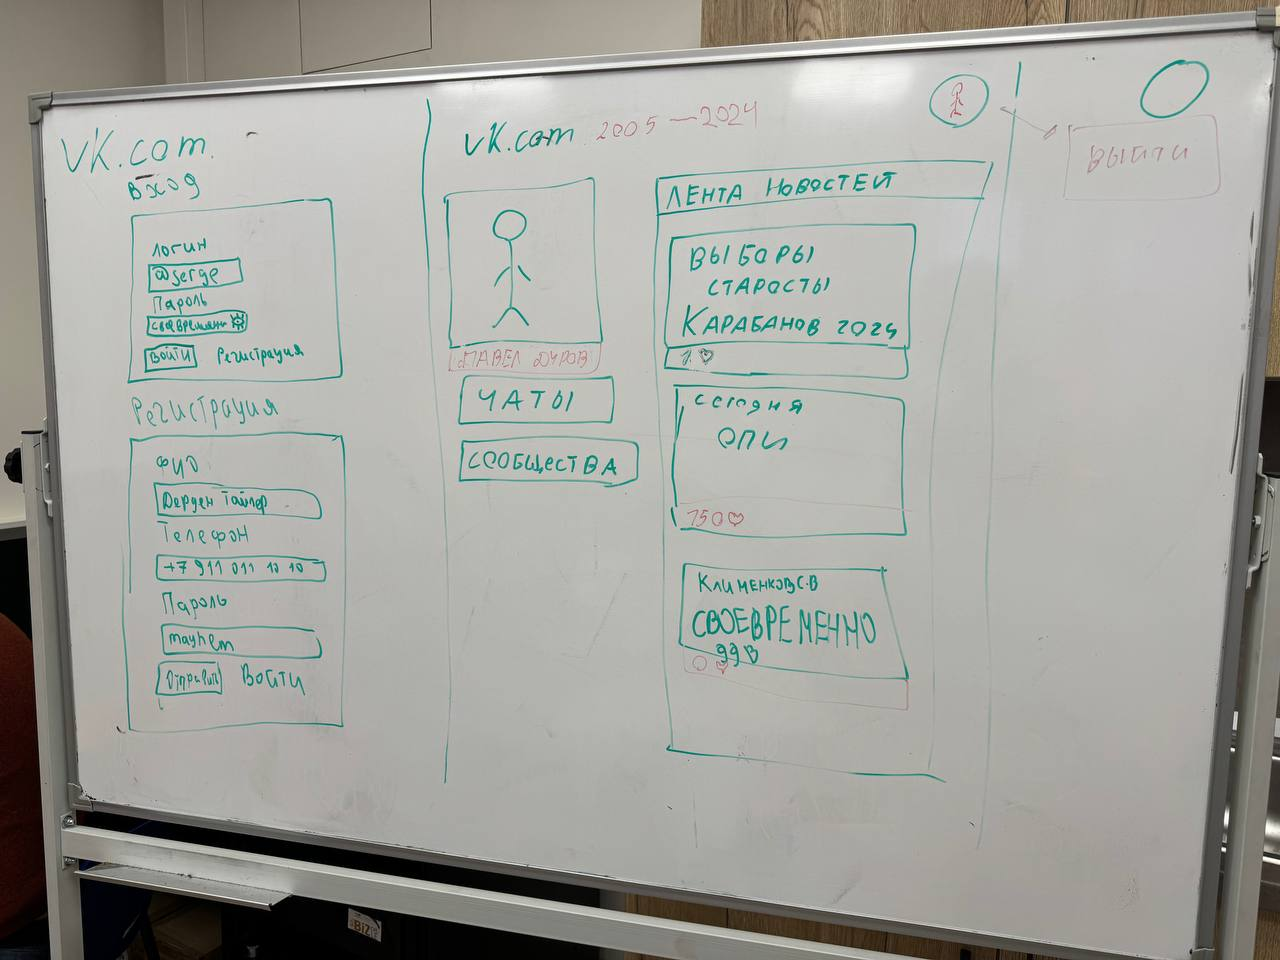
\includegraphics{./img/prototype.jpg}}
  \caption{Прототип интерфейса}
\end{figure}
